% ********** Chapter 2 **********
\chapter{Binaire zoekboom}
\label{sec:Hoofdstuk 2}

\begin{figure}[h]
	\centering
		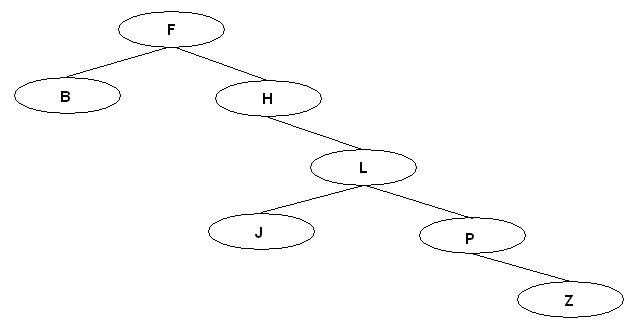
\includegraphics[width=\textwidth]{chap2/binarytree}
	\label{fig:binarytree}
\end{figure}

\section{Introductie}
Een van de simpelste zoekbomen is de binaire zoekboom. Elke interne knoop heeft twee kinderen waarvan de linkerkant lager is en de rechterkant hoger is dan de waarde in de interne knoop.\\
\\
\section{Zoeken}
Bij het zoeken naar een waarde $k$ in een binaire boom wordt begonnen in de root knoop. Als $k$ kleiner is dan de waarde in de knoop $p$ wordt verder gezocht in het linkerkind van $p$. Wanneer $k$ groter is dan de waarde in $p$ wordt verder gezocht in het rechterkind van $p$. Dit wordt gedaan tot een externe knoop is bereikt of wanneer $k$ gevonden is.\\
\\
\section{Toevoegen}
Met behulp van bovenstaande zoek methode wordt gezocht naar de toe te voegen waarde $k$. Wanneer de gevonden waarde $p$ een interne knoop is wordt er direct gestopt met toevoegen, $k$ zit namelijk al in de boom. Wanneer $p$ een externe knoop is wordt deze vervangen door $k$ en worden twee externe kinderen toegevoegd aan $k$.\\
\\
\section{Analyse}

% ********** End of chapter **********